% !TeX program = xelatex
\documentclass[a4paper,10pt]{article}

% ============================================================================
% សន្លឹកកិច្ចការសិស្ស ស-ខ្មៅ (Student Guided-Inquiry Worksheet - Grade 8 13.2.4 SQMID1)
% បរិបទ៖ ថ្នាក់រៀនគ្មានស្លាយ LCD – ការេ និងគន្លឹះ Polya បន្លាយអង្កត់ទ្វេដង ២ ទំព័រ A4
% ============================================================================
\usepackage[a4paper, left=0.90cm, right=0.90cm, top=0.75cm, bottom=0.85cm, footskip=0.45cm]{geometry}
\usepackage{amsmath, amssymb}
\usepackage{unicode-math}
\usepackage{fontspec}
\usepackage{array, colortbl}
\usepackage[table]{xcolor}
\usepackage{enumitem}
\usepackage{pifont}
\usepackage{fancyhdr}
\usepackage{lastpage}
\usepackage{tikz}
\usepackage[most]{tcolorbox}
\usetikzlibrary{calc, arrows.meta, angles, quotes, decorations.markings, positioning, babel}

\makeatletter
\let\@expl@@@mark@update@singlecol@structures@@\relax
\makeatother

\providecommand{\NGSFindFonts}{%
  \IfFileExists{C:/Windows/Fonts/cambria.ttc}{%
    \def\NGSSysPath{C:/Windows/Fonts/}%
    \def\NGSUserPath{C:/Users/KIT/AppData/Local/Microsoft/Windows/Fonts/}%
  }{%
    \IfFileExists{./fonts/KhmerOSsiemreap.ttf}{\def\NGSSysPath{./fonts/}\def\NGSUserPath{./fonts/}}{%
    \IfFileExists{../fonts/KhmerOSsiemreap.ttf}{\def\NGSSysPath{../fonts/}\def\NGSUserPath{../fonts/}}{%
    \IfFileExists{../../fonts/KhmerOSsiemreap.ttf}{\def\NGSSysPath{../../fonts/}\def\NGSUserPath{../../fonts/}}{%
    \IfFileExists{../../../fonts/KhmerOSsiemreap.ttf}{\def\NGSSysPath{../../../fonts/}\def\NGSUserPath{../../../fonts/}}{%
    \IfFileExists{../../../../fonts/KhmerOSsiemreap.ttf}{\def\NGSSysPath{../../../../fonts/}\def\NGSUserPath{../../../../fonts/}}{%
    \IfFileExists{../../../../../fonts/KhmerOSsiemreap.ttf}{\def\NGSSysPath{../../../../../fonts/}\def\NGSUserPath{../../../../../fonts/}}{%
    \IfFileExists{../../../../../../fonts/KhmerOSsiemreap.ttf}{\def\NGSSysPath{../../../../../../fonts/}\def\NGSUserPath{../../../../../../fonts/}}{%
      \def\NGSSysPath{../../../../../../../fonts/}\def\NGSUserPath{../../../../../../../fonts/}%
    }}}}}}}%
  }%
}
\NGSFindFonts

\setmathfont[Path={\NGSSysPath}, FontIndex=1, Scale=1.02]{cambria.ttc}
\defaultfontfeatures{Ligatures=TeX}

\setmainfont[
  Path={\NGSUserPath},
  Extension=.ttf,
  Script=Khmer,
  BoldFont={KhmerOSsiemreap},
  BoldFeatures={FakeBold=1.8},
  ItalicFont={KhmerOSsiemreap},
  ItalicFeatures={FakeSlant=0.25},
  BoldItalicFont={KhmerOSsiemreap},
  BoldItalicFeatures={FakeBold=1.8, FakeSlant=0.25}
]{KhmerOSsiemreap}

\newfontfamily\muol[Path={\NGSUserPath}, Extension=.ttf, Script=Khmer]{KhmerOSmuollight}
\newfontfamily\TimesEn[Path={\NGSSysPath}, Extension=.ttf, BoldFont={timesbd}, ItalicFont={timesi}, BoldItalicFont={timesbi}]{times}

\XeTeXlinebreaklocale "km"
\XeTeXlinebreakskip = 0pt plus 1pt minus 0.1pt

\definecolor{panelgray}{gray}{0.94}
\definecolor{headgray}{gray}{0.86}
\definecolor{subgray}{gray}{0.91}

\pagestyle{fancy}
\fancyhf{}
\renewcommand{\headrulewidth}{0pt}
\fancyfoot[L]{\fontsize{8pt}{10pt}\selectfont អនុវិទ្យាល័យព្រះក្រសាំង \en{|} គណិតវិទ្យា ថ្នាក់ទី៨ \en{|} មេរៀនទី១៣ (២.៤ ការេ និងទ្រឹស្ដីបទចំណុចកណ្ដាល)}
\fancyfoot[R]{\fontsize{8.2pt}{10pt}\selectfont ទំព័រ \en{\thepage\ / \pageref{LastPage}}}

\setlength{\parindent}{0pt}
\setlength{\parskip}{0pt}
\setlength{\tabcolsep}{4pt}

\newcommand{\en}[1]{{\TimesEn #1}}
\newcommand{\enbf}[1]{{\TimesEn\textbf{#1}}}
\newcommand{\unit}[1]{\,\text{\en{#1}}}
\newcommand{\cnum}[1]{{\fontsize{10pt}{12pt}\selectfont\ding{\numexpr171+#1\relax}}}
\newcommand{\chk}{\tikz[baseline=-0.15ex]\draw[black, line width=0.8pt] (0,0) rectangle (0.25cm,0.25cm);}
\newcommand{\tri}[1]{\ensuremath{\triangle #1}}
\newcommand{\ang}[1]{\ensuremath{\angle #1}}
\newcommand{\cg}{\ensuremath{\cong}}
\newcommand{\dotline}[1]{\makebox[#1]{\dotfill}}

\newcolumntype{L}[1]{>{\raggedright\arraybackslash}p{#1}}
\newcolumntype{C}[1]{>{\centering\arraybackslash}p{#1}}

\tikzset{
  tk1/.style={postaction={decorate},decoration={markings,mark=at position 0.50 with {\draw[black, line width=0.90pt](0,-0.095)--(0,0.095);}}},
  tk2/.style={postaction={decorate},decoration={markings,
    mark=at position 0.45 with {\draw[black, line width=0.90pt](0,-0.095)--(0,0.095);},
    mark=at position 0.55 with {\draw[black, line width=0.90pt](0,-0.095)--(0,0.095);}}},
  par1/.style={postaction={decorate},decoration={markings,mark=at position 0.52 with {\draw[black, line width=0.90pt](-0.07,0.08)--(0.05,0)--(-0.07,-0.08);}}}
}

\newcommand{\secbar}[2]{%
  \vspace{3pt}
  \noindent\colorbox{headgray}{\parbox{\dimexpr\linewidth-2\fboxsep\relax}{%
    \vspace{1.5pt}{\muol\fontsize{9.5pt}{13.5pt}\selectfont #1}\hfill{\fontsize{8.5pt}{12pt}\selectfont\textbf{#2}}\vspace{1.5pt}%
  }}\par\vspace{3pt}
}

\begin{document}
\fontsize{9.5pt}{14.3pt}\selectfont

% ============================================================================
% ទំព័រទី១៖ E1 ទស្សន៍ទាយ + E2 វាស់ខ្នាតពិត 1:1 & គន្លឹះ Polya បន្លាយអង្កត់ទ្វេដង
% ============================================================================
\begin{tcolorbox}[enhanced, sharp corners, colback=white, colframe=black, boxrule=1.0pt, top=4pt, bottom=4pt, left=6pt, right=6pt]
  \begin{center}
    {\muol\fontsize{10.5pt}{15pt}\selectfont សន្លឹកកិច្ចការសិស្ស — មេរៀនទី១៣៖ ចតុកោណ \enbf{(}២.៤ ការេ និងទ្រឹស្ដីបទចំណុចកណ្ដាល\enbf{)}}\\[2pt]
    {\footnotesize សៀវភៅសិក្សាគោលថ្នាក់ទី៨ ទំព័រ ១៧៩--១៨១ និង ១៨៥--១៨៦ \en{|} គន្លឹះ \en{Polya} បន្លាយអង្កត់ទ្វេដង (គ្មានស្លាយ \en{LCD})}
  \end{center}
  \vspace{2pt}
  \hrule height 0.5pt
  \vspace{4pt}
  ឈ្មោះសិស្សទី១៖ \dotline{3.6cm} \hspace{0.15cm} ឈ្មោះដៃគូទី២៖ \dotline{3.6cm} \hspace{0.15cm} ថ្នាក់ទី៨៖ \dotline{1.0cm} \hspace{0.15cm} ថ្ងៃទី១៧/១២/២០២៦
\end{tcolorbox}

% --- E1 Engage ---
\secbar{ផ្នែកទី១ ៖ បេសកកម្មផ្ដើមមេរៀន — វាស់ទទឹងបឹង និងជន្ទល់ដំបូលកែង \enbf{(E1 -- Engage)}}{៣ នាទី}
\begin{tcolorbox}[enhanced, sharp corners, colback=panelgray, colframe=black, boxrule=0.7pt, top=3.5pt, bottom=3.5pt, left=6pt, right=6pt]
  $\bullet$ \textbf{បញ្ហាទី១ (វាស់ទទឹងបឹង $BC$)៖} កសិករបោះបង្គោល $A$ លើគោក រកចំណុចកណ្ដាល $D$ នៃ $AB$ និង $E$ នៃ $AC$ វាស់បាន $DE = 18\unit{m}$ ។ តើទទឹងបឹង $BC$ ស្មើប៉ុន្មានម៉ែត្រ? \hspace{0.2cm} \chk\ $18\unit{m}$ \hspace{0.4cm} \chk\ $27\unit{m}$ \hspace{0.4cm} \chk\ $36\unit{m}$\par\vspace{1.5pt}
  $\bullet$ \textbf{បញ្ហាទី២ (ជន្ទល់ដំបូល)៖} ជាងដែកផ្សារធ្នឹមត្រីកោណ $\tri{ABC}$ ដោយដាក់ជន្ទល់កណ្ដាល $BO = OA = OC$ ($O$ កណ្ដាល $AC$) ។ តើមុំកំពូលដំបូល $\ang{ABC}$ ស្មើប៉ុន្មានដឺក្រេ? \hspace{0.2cm} \chk\ $60^\circ$ \hspace{0.4cm} \chk\ $90^\circ$ \hspace{0.4cm} \chk\ $120^\circ$
\end{tcolorbox}

% --- E2 Explore ---
\secbar{ផ្នែកទី២ ៖ វាស់ខ្នាតពិត \enbf{1:1} និងគន្លឹះ \enbf{Polya} បន្លាយអង្កត់ទ្វេដង \enbf{(E2 -- Explore)}}{១១ នាទី}
\textbf{សកម្មភាពទី១ (៤ នាទី)៖} ប្រើបន្ទាត់ក្រិតវាស់ប្រវែងពិត $1:1$ នៃបាតមធ្យម $DE$ និងមេដ្យានត្រីកោណកែង $QO$ ខាងក្រោម៖\par\vspace{3pt}
\begin{tabular}{@{}C{7.20cm} L{11.40cm}@{}}
  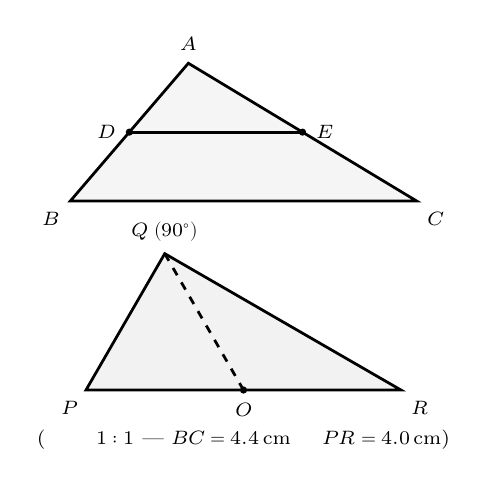
\begin{tikzpicture}[x=1cm, y=1cm, baseline={(0,2.75)}, every node/.style={font=\scriptsize, text=black}]
    % ខាងលើ៖ ត្រីកោណ ABC មាន BC = 4.4 cm => DE = 2.2 cm
    \begin{scope}[shift={(0,1.85)}]
      \coordinate (B) at (0,0); \coordinate (C) at (4.4,0);
      \coordinate (A) at (1.5,1.75);
      \coordinate (D) at ($(A)!0.5!(B)$); \coordinate (E) at ($(A)!0.5!(C)$);
      \fill[gray!8] (A)--(B)--(C)--cycle;
      \draw[line width=1.0pt] (A)--(B)--(C)--cycle;
      \draw[line width=1.05pt] (D)--(E);
      \fill (D) circle (1.3pt) node[left=1.5pt] {$D$};
      \fill (E) circle (1.3pt) node[right=1.5pt] {$E$};
      \node[above=1pt] at (A) {$A$}; \node[below left=0.5pt] at (B) {$B$}; \node[below right=0.5pt] at (C) {$C$};
    \end{scope}
    % ខាងក្រោម៖ ត្រីកោណកែង PQR មាន PR = 4.0 cm => មេដ្យាន QO = 2.0 cm
    \begin{scope}[shift={(0.20,-0.55)}]
      \coordinate (P) at (0,0); \coordinate (R) at (4.0,0); \coordinate (O) at (2.0,0);
      \coordinate (Q) at ({2.0 + 2.0*cos(120)}, {2.0*sin(120)});
      \fill[gray!10] (P)--(Q)--(R)--cycle;
      \draw[line width=1.0pt] (P)--(Q)--(R)--cycle;
      \draw[line width=1.0pt, dashed] (Q)--(O);
      \fill (O) circle (1.3pt) node[below=1pt] {$O$};
      \node[above=1pt] at (Q) {$Q\;(90^\circ)$}; \node[below left=0.5pt] at (P) {$P$}; \node[below right=0.5pt] at (R) {$R$};
      \node[anchor=north, font=\scriptsize] at (2.0,-0.38) {(ខ្នាតពិត $1:1$ — $BC=4.4\unit{cm}$ និង $PR=4.0\unit{cm}$)};
    \end{scope}
  \end{tikzpicture}
  &
  {\renewcommand{\arraystretch}{1.32}
  \begin{tabular}{|L{4.80cm}|L{5.80cm}|}
    \hline
    \rowcolor{subgray}\textbf{ធាតុដែលត្រូវវាស់ និងសង្កេត} & \textbf{លទ្ធផលវាស់ និងសន្និដ្ឋាន} \\
    \hline
    បាតមធ្យម $DE$ ធៀបនឹង $BC=4.4\unit{cm}$ & $DE = \dotline{1.2cm}\unit{cm} = \dfrac{1}{\dotline{0.5cm}} BC$ \\
    \hline
    ទិសដៅនៃបន្ទាត់ $DE$ និងជ្រុង $BC$ & $DE \dotline{1.0cm} BC$ (\chk\ ស្របគ្នា) \\
    \hline
    វាស់មេដ្យាន $QO$ ក្នុង $\tri{PQR}$ កែងត្រង់ $Q$ & $QO = \dotline{1.2cm}\unit{cm}$ ($PR=4.0\unit{cm}$) \\
    \hline
    ធៀបមេដ្យាន $QO$ ទៅនឹងអ៊ីប៉ូតេនុស $PR$ & $QO = OP = OR = \dfrac{1}{\dotline{0.5cm}} PR$ \\
    \hline
    ក្នុង\textbf{ការេ} $ABCD$ (ផ្ចិត $O$) & $AC=BD, AC\perp BD$, មុំពុះ $=\dotline{0.9cm}^\circ$ \\
    \hline
  \end{tabular}}
\end{tabular}

\vspace{6pt}
\textbf{សកម្មភាពទី២ — គន្លឹះ \en{Polya} «បន្លាយអង្កត់ទ្វេដង» ស្រាយបញ្ជាក់ទ្រឹស្ដីបទ (៧ នាទី)៖} បំពេញចន្លោះតាមរូបសៀវភៅគោល ទំ.១៨០--១៨១៖\par\vspace{3pt}
{\renewcommand{\arraystretch}{1.24}
\begin{tabular}{|L{9.15cm}|L{9.15cm}|}
  \hline
  \rowcolor{subgray}\textbf{ផ្នែក ក៖ ទ្រឹស្ដីបទទី១ — បាតមធ្យមត្រីកោណ ($DE=\frac{1}{2}BC$, ទំ.១៨០)} & \textbf{ផ្នែក ខ៖ ទ្រឹស្ដីបទទី៣--៤ — មេដ្យានត្រីកោណកែង ($BO=\frac{1}{2}AC$, ទំ.១៨១)} \\
  \hline
  \begin{center}
  \vspace{-1pt}
  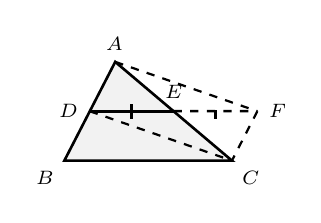
\begin{tikzpicture}[scale=0.76, every node/.style={font=\scriptsize}]
    \coordinate (B) at (0,0); \coordinate (C) at (2.80,0);
    \coordinate (A) at (0.85,1.65);
    \coordinate (D) at ($(A)!0.5!(B)$); \coordinate (E) at ($(A)!0.5!(C)$);
    \coordinate (F) at ($(E)!-1!(D)$);
    \fill[gray!10] (A)--(B)--(C)--cycle;
    \draw[line width=0.95pt] (A)--(B)--(C)--cycle;
    \draw[line width=0.95pt, tk1] (D)--(E);
    \draw[line width=0.9pt, dashed, tk1] (E)--(F);
    \draw[line width=0.8pt, dashed] (A)--(F) (F)--(C) (D)--(C);
    \node[above=0.5pt] at (A) {$A$}; \node[below left=0.5pt] at (B) {$B$}; \node[below right=0.5pt] at (C) {$C$};
    \node[left=1pt] at (D) {$D$}; \node[above=1pt] at (E) {$E$}; \node[right=1pt] at (F) {$F$};
  \end{tikzpicture}
  \vspace{-2pt}
  \end{center}
  ១. បន្លាយ $DE$ ឱ្យបាន $DE = EF$៖ ចតុកោណ $ADCF$ មានអង្កត់ទ្រូងកាត់គ្នាត្រង់ចំណុចកណ្ដាល $E$ ជា \dotline{2.3cm}\par
  $\Rightarrow AD = \dotline{1.0cm}$ និង $AB \parallel CF$ ។\par
  ២. តែ $AD = DB \Rightarrow DB = \dotline{1.0cm}$ និង $DB \parallel CF$\par
  $\Rightarrow$ ចតុកោណ $BDFC$ ជា \dotline{2.3cm} ដែរ!\par
  ៣. ដូច្នេះ $DE \parallel \dotline{0.9cm}$ និង $DE = \frac{1}{2}DF = \frac{1}{2}\dotline{0.9cm}$ ។
  &
  \begin{center}
  \vspace{-1pt}
  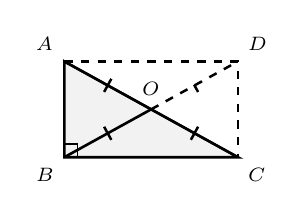
\begin{tikzpicture}[scale=0.76, every node/.style={font=\scriptsize}]
    \coordinate (B) at (0,0); \coordinate (C) at (2.90,0);
    \coordinate (A) at (0,1.60); \coordinate (D) at (2.90,1.60);
    \coordinate (O) at (1.45,0.80);
    \fill[gray!10] (A)--(B)--(C)--cycle;
    \draw[line width=0.95pt] (A)--(B)--(C)--cycle;
    \draw[line width=0.8pt, dashed] (A)--(D)--(C);
    \draw[line width=0.95pt, tk1] (B)--(O);
    \draw[line width=0.9pt, dashed, tk1] (O)--(D);
    \draw[line width=0.85pt, tk1] (A)--(O); \draw[line width=0.85pt, tk1] (O)--(C);
    \draw[line width=0.65pt] (0,0.22)--(0.22,0.22)--(0.22,0);
    \node[above left=0.5pt] at (A) {$A$}; \node[below left=0.5pt] at (B) {$B$};
    \node[below right=0.5pt] at (C) {$C$}; \node[above right=0.5pt] at (D) {$D$};
    \node[above=1.5pt] at (O) {$O$};
  \end{tikzpicture}
  \vspace{-2pt}
  \end{center}
  ១. បន្លាយមេដ្យាន $BO$ ឱ្យបាន $BO = OD$៖ ចតុកោណ $ABCD$ មាន $OA=OC, OB=OD$ ជា \dotline{2.3cm}\par
  ២. \textbf{ទ្រឹស្ដីបទទី៣៖} បើ $\ang{ABC}=90^\circ$ នោះ $ABCD$ ជា \dotline{2.1cm}\par
  $\Rightarrow$ អង្កត់ទ្រូង $BD = \dotline{1.0cm} \Rightarrow BO = \frac{1}{2}\dotline{1.0cm}$ ។\par
  ៣. \textbf{ទ្រឹស្ដីបទទី៤ (ច្រាស)៖} បើ $BO=\frac{1}{2}AC$ នោះ $BD=2BO=\dotline{1.0cm}$\par
  $\Rightarrow ABCD$ ជាចតុកោណកែង $\Rightarrow \ang{ABC} = \dotline{0.9cm}^\circ$ ។ \\
  \hline
\end{tabular}}

\newpage

% ============================================================================
% ទំព័រទី២៖ E3 ធនាគារហេតុផល ①–⑤ + E4 លំហាត់គំរូ ២ + E5 ប្រតិបត្តិ & Exit Check + កិច្ចការផ្ទះ
% ============================================================================
\secbar{ផ្នែកទី៣ ៖ សង្ខេបលក្ខណៈការេ និងធនាគារហេតុផល \cnum{1}--\cnum{5} \enbf{(E3 -- Explain)}}{៦ នាទី}
\begin{tcolorbox}[enhanced, sharp corners, colback=white, colframe=black, boxrule=0.8pt, top=4pt, bottom=4pt, left=6pt, right=6pt]
  \cnum{1} \textbf{ការេ៖} មានជ្រុងទាំង ៤ ប៉ុនគ្នា, មុំកែង ៤, អង្កត់ទ្រូងប៉ុនគ្នា កែងគ្នាត្រង់ចំណុចកណ្ដាល និងពុះមុំជា \dotline{1.1cm}$^\circ$ (អ័ក្សឆ្លុះ ៤) ។\par\vspace{2pt}
  \cnum{2} \textbf{ទ្រឹស្ដីបទទី១ (បាតមធ្យមត្រីកោណ)៖} បើ $D, E$ កណ្ដាលនៃ $AB, AC$ នោះ $DE \parallel \dotline{1.0cm}$ និង $DE = \frac{1}{2}\dotline{1.0cm}$ ។\par\vspace{2pt}
  \cnum{3} \textbf{ទ្រឹស្ដីបទទី២៖} បន្ទាត់តាមចំណុចកណ្ដាលជ្រុងទី១ ហើយស្របនឹងជ្រុងទី២ ត្រូវកាត់តាម \dotline{2.6cm} នៃជ្រុងទី៣ ។\par\vspace{2pt}
  \cnum{4} \textbf{ទ្រឹស្ដីបទទី៣ (មេដ្យានត្រីកោណកែង)៖} ក្នុងត្រីកោណកែង មេដ្យានចំពោះអ៊ីប៉ូតេនុសស្មើនឹង \dotline{2.8cm} ($BO=\frac{1}{2}AC$) ។\par\vspace{2pt}
  \cnum{5} \textbf{ទ្រឹស្ដីបទទី៤ (សម្គាល់ត្រីកោណកែង)៖} បើមេដ្យាន $BO = \frac{1}{2}AC$ នោះត្រីកោណ $\tri{ABC}$ កែងត្រង់កំពូល \dotline{1.0cm} ។
\end{tcolorbox}

% --- E4 Elaborate ---
\secbar{ផ្នែកទី៤ ៖ លំហាត់គំរូអនុវត្ត និងធនាគារហេតុផល \cnum{1}--\cnum{5} \enbf{(E4 -- Elaborate)}}{១០ នាទី}
{\renewcommand{\arraystretch}{1.24}
\begin{tabular}{|L{9.15cm}|L{9.15cm}|}
  \hline
  \rowcolor{subgray}\textbf{គំរូទី១ (លំហាត់ទី៨ ទំ.១៨៦ — បាតមធ្យមត្រីកោណ)} & \textbf{គំរូទី២ (មេដ្យានត្រីកោណកែង និងអង្កត់ទ្រូងការេ)} \\
  \hline
  ក្នុងត្រីកោណ $ABC$ ចំណុច $D, E$ ជាចំណុចកណ្ដាលនៃ $AB, AC$ ។ បើ $DE = 9x - 4$ និង $BC = 6x + 4$ គណនាតម្លៃ $x, DE$ និង $BC$ ។\par
  \begin{center}
  \vspace{-1pt}
  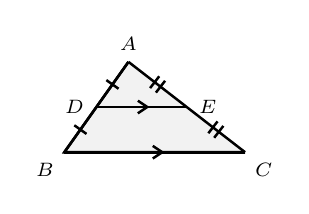
\begin{tikzpicture}[scale=0.74, every node/.style={font=\scriptsize}]
    \coordinate (B) at (0,0); \coordinate (C) at (3.10,0);
    \coordinate (A) at (1.10,1.55);
    \coordinate (D) at ($(A)!0.5!(B)$); \coordinate (E) at ($(A)!0.5!(C)$);
    \fill[gray!10] (A)--(B)--(C)--cycle;
    \draw[line width=0.95pt] (A)--(B)--(C);
    \draw[line width=0.9pt, tk1] (A)--(D); \draw[line width=0.9pt, tk1] (D)--(B);
    \draw[line width=0.9pt, tk2] (A)--(E); \draw[line width=0.9pt, tk2] (E)--(C);
    \draw[line width=0.95pt, par1] (D)--(E); \draw[line width=0.95pt, par1] (B)--(C);
    \node[above=0.5pt] at (A) {$A$}; \node[below left=0.5pt] at (B) {$B$}; \node[below right=0.5pt] at (C) {$C$};
    \node[left=1pt] at (D) {$D$}; \node[right=1pt] at (E) {$E$};
  \end{tikzpicture}
  \vspace{-1pt}
  \end{center}
  $\bullet$ តាម \cnum{2} គេមានសមីការ៖ $BC = 2 \cdot DE$\par
  $\Rightarrow 6x + 4 = 2(\dotline{2.0cm}) \Rightarrow 6x + 4 = \dotline{2.2cm}$\par
  $\Rightarrow 12x = \dotline{1.2cm} \Rightarrow x = \dotline{1.0cm}$\par
  $\bullet$ ប្រវែង៖ $DE = \dotline{1.4cm}$ និង $BC = \dotline{1.4cm}$ ។
  &
  (ក) $\tri{ABC}$ កែងត្រង់ $B$ មានមេដ្យាន $BO=6.5\unit{cm}$ និង $\ang{ACB}=28^\circ$ ។ រក $AC$ និង $\ang{OBC}$ ។ (ខ) ការេ $MNPQ$ មានអង្កត់ទ្រូង $MP=8\unit{cm}$ កាត់ $NQ$ ត្រង់ $I$ ។ រក $IN$ និង $\ang{IMN}$ ។\par
  \begin{center}
  \vspace{-1pt}
  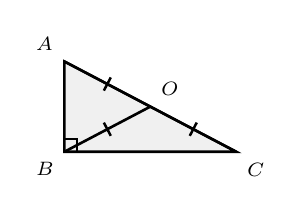
\begin{tikzpicture}[scale=0.74, every node/.style={font=\scriptsize}]
    \coordinate (B) at (0,0); \coordinate (C) at (2.95,0);
    \coordinate (A) at (0,1.55); \coordinate (O) at (1.475,0.775);
    \fill[gray!12] (A)--(B)--(C)--cycle;
    \draw[line width=0.95pt] (A)--(B)--(C)--cycle;
    \draw[line width=0.9pt, tk1] (A)--(O); \draw[line width=0.9pt, tk1] (O)--(C);
    \draw[line width=0.95pt, tk1] (B)--(O);
    \draw[line width=0.65pt] (0,0.22)--(0.22,0.22)--(0.22,0);
    \node[above left=0.5pt] at (A) {$A$}; \node[below left=0.5pt] at (B) {$B$};
    \node[below right=0.5pt] at (C) {$C$}; \node[above right=0.5pt] at (O) {$O$};
  \end{tikzpicture}
  \vspace{-1pt}
  \end{center}
  $\bullet$ (ក) តាម \cnum{4}៖ $AC = 2 \cdot BO = \dotline{1.5cm}\unit{cm}$\par
  $\bullet$ ដោយ $OB=OC \Rightarrow \tri{OBC}$ សមបាត $\Rightarrow \ang{OBC}=\dotline{1.0cm}^\circ$\par
  $\bullet$ (ខ) ក្នុងការេ (\cnum{1})៖ $IN = \frac{1}{2}MP = \dotline{1.2cm}\unit{cm}$, $\ang{IMN}=\dotline{0.9cm}^\circ$ ។ \\
  \hline
\end{tabular}}\par\vspace{3pt}
$\bullet$ \textbf{ឆ្លុះបញ្ចាំង (\en{EIA})៖} ក្នុងត្រីកោណកែង $\tri{ABC}$ មេដ្យាន $BO$ ចែកត្រីកោណជាត្រីកោណ \dotline{2.6cm} ចំនួន ២ គឺ $\tri{OAB}$ និង $\tri{OBC}$!

% --- E5 Evaluate ---
\secbar{ផ្នែកទី៥ ៖ លំហាត់ប្រតិបត្តិ ផ្ទៀងផ្ទាត់ជាដៃគូ និង \enbf{Exit Check (E5 -- Evaluate)}}{១០ នាទី}
\begin{tabular}{@{}L{13.15cm} C{5.65cm}@{}}
  \textbf{១.} ក្នុង $\tri{ABC}$ មាន $AB=12\unit{cm}, BC=16\unit{cm}, AC=20\unit{cm}$ ហើយ $D, E, F$ ជាចំណុចកណ្ដាលនៃ $AB, AC, BC$ ។ គណនាប្រវែង $DE, EF, DF$ និងបរិមាត្រនៃ $\tri{DEF}$៖\par\vspace{3pt}
  $DE=\dotline{1.3cm}, EF=\dotline{1.3cm}, DF=\dotline{1.3cm} \Rightarrow P_{\tri{DEF}} = \dotline{2.2cm}\unit{cm}$\par\vspace{4pt}
  \textbf{២.} ក្នុង $\tri{KLM}$ មេដ្យាន $KO=7\unit{cm}$ និងជ្រុង $LM=14\unit{cm}$ ។ ប្រភេទនៃ $\tri{KLM}$៖ \dotline{3.0cm}\par\vspace{4pt}
  \textbf{៣. បិទបញ្ហា E1៖} ទទឹងបឹង $BC = \dotline{1.5cm}\unit{m}$ (តាម \cnum{2}) ហើយដំបូលកែងត្រង់ $B$ (តាម \cnum{5})!
  &
  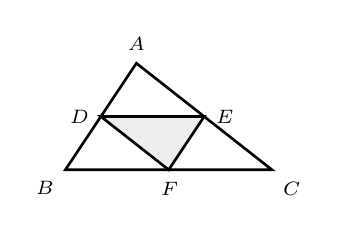
\begin{tikzpicture}[scale=0.82, baseline={(0,1.45)}, every node/.style={font=\scriptsize}]
    \coordinate (B) at (0,0); \coordinate (C) at (3.20,0);
    \coordinate (A) at (1.10,1.65);
    \coordinate (D) at ($(A)!0.5!(B)$);
    \coordinate (E) at ($(A)!0.5!(C)$);
    \coordinate (F) at ($(B)!0.5!(C)$);
    \fill[gray!14] (D)--(E)--(F)--cycle;
    \draw[line width=0.95pt] (A)--(B)--(C)--cycle;
    \draw[line width=0.95pt] (D)--(E)--(F)--cycle;
    \node[above=1pt] at (A) {$A$}; \node[below left=1pt] at (B) {$B$}; \node[below right=1pt] at (C) {$C$};
    \node[left=1pt] at (D) {$D$}; \node[right=1pt] at (E) {$E$}; \node[below=1pt] at (F) {$F$};
  \end{tikzpicture}
\end{tabular}

\vspace{4pt}
\begin{tcolorbox}[enhanced, sharp corners, colback=panelgray, colframe=black, boxrule=0.8pt, top=4pt, bottom=4pt, left=6pt, right=6pt]
  \textbf{ខ. សំណួរត្រួតពិនិត្យរហ័ស (\en{Exit Check} — គូសរង្វង់ចម្លើយត្រឹមត្រូវតែ ១)៖}\par
  (១) មុំរវាងអង្កត់ទ្រូង និងជ្រុងនៃការេស្មើប៉ុន្មាន? (២) ត្រីកោណកែងមានអ៊ីប៉ូតេនុស $18\unit{cm}$ តើមេដ្យានចំពោះអ៊ីប៉ូតេនុសស្មើប៉ុន្មាន?\par\vspace{2pt}
  \hspace*{0.2cm}\textbf{A.} $90^\circ$ និង $9\unit{cm}$ \hspace{1.0cm} \textbf{B.} $45^\circ$ និង $18\unit{cm}$ \hspace{1.0cm} \textbf{C.} $45^\circ$ និង $9\unit{cm}$ \hspace{1.0cm} \textbf{D.} $60^\circ$ និង $9\unit{cm}$
\end{tcolorbox}

% --- Step 5 Homework ---
\secbar{ផ្នែកទី៦ ៖ កិច្ចការផ្ទះ និងបណ្ដាំផ្ញើ \enbf{(}ទំព័រ ១៨៥--១៨៦\enbf{)}}{ធ្វើក្នុងសៀវភៅកិច្ចការផ្ទះ}
$\bullet$ \textbf{លំហាត់ទី១ (លំហាត់ទី២ ទំ.១៨៥)៖} សង់ការេ $ABCD$ ដោយស្គាល់ប្រវែងអង្កត់ទ្រូង $AC = 6\unit{cm}$ (គូស $AC=BD=6\unit{cm}$ កែងគ្នាត្រង់ចំណុចកណ្ដាល $O$) ។\par\vspace{2pt}
$\bullet$ \textbf{លំហាត់ទី២៖} ក្នុង $\tri{ABC}$ ចំណុច $D$ ជាចំណុចកណ្ដាលនៃ $AB$ ហើយបន្ទាត់តាម $D$ ស្របនឹង $BC$ កាត់ $AC$ ត្រង់ $E$ ។ បើ $AE=5\unit{cm}, DE=3x+2\unit{cm}$ និង $BC=16\unit{cm}$ ចូរគណនាប្រវែង $AC$ និងតម្លៃ $x$ រួចអានជាមុន \textbf{២.៥ លក្ខណៈចតុកោណព្នាយ} (ទំ.១៨១--១៨៤) ។

\end{document}
